\chapter{Zastosowane podejście}
\label{c4}

W niniejszym rozdziale zawarto opis zastosowanego podejścia, do porównania programowania wizualnego i programowania natywnego.

\section{Wstęp}
\label{c41}

Zastosowane podejście polegało na stworzeniu jak największej ilości aplikacji, wykorzystujących różne komponenty. Następnie należało wykreować analogiczne aplikacje w języku Java. Dysponując obszerną, pokrywającą niemal wszystkie możliwości App Inventora  liczbą aplikacji programista jest w stanie udzielić odpowiedzi na wiele pytań dotyczących tego narzędzia, postawionych we wstępie pracy. (\ref{c12})

\section{Dalvik Debug Monitor}

Na poniższym obrazku widać narzędzie Dalvik Debug Monitor. Na telefonie uruchomione są dwa dodatkowe, poza systemowymi, procesy jednocześnie. Po prawej stronie widać wykres obciążenia procesora, poszczególnych procesów.

\begin{figure}[H] 
\centering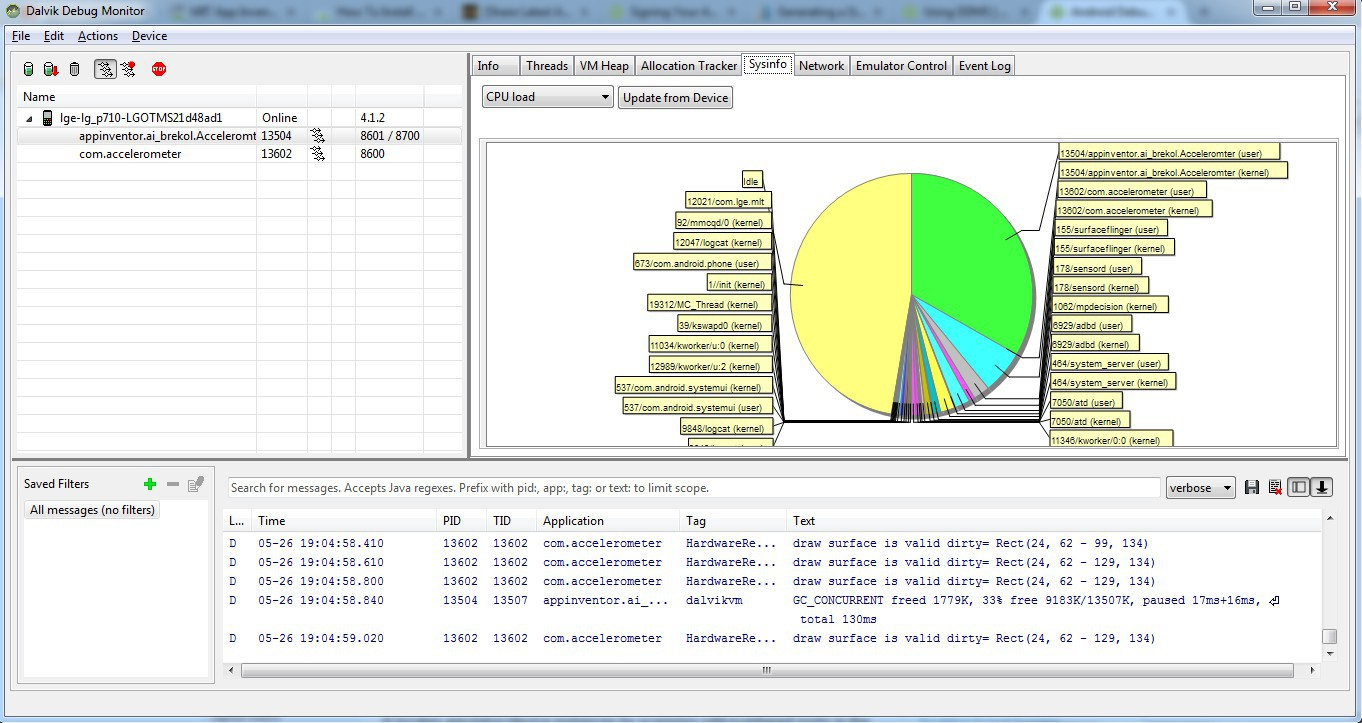
\includegraphics[width=12cm]{figures/dalvik}
\caption{Przykładowy zrzut ekranu DDMS}
\end{figure}



\subsection{Uruchamianie aplikacji w androidzie}
W systemie Android każda aplikacja jest uruchamiana w osobnym procesie, a każdy z procesów działa na swojej własnej wirtualnej maszynie. Każda z tych wirtualnych maszyn wystawia unikalny port, do którego może się podłączyć debbuger. Dalvik Debug Monitor (\ref{ddms}) zaraz po starcie podłącza się do Android Debug Bridge (ADB) - narzędzia, które pozwala na komunikację z podłączonym urządzeniem (\ref{adb}).

\subsection{Połączenie ADB - DDMS}

Po podłączeniu urządzenia tworzony jest serwis monitorujący pomiędzy ADB a DDMS, który powiadamia DDMS, kiedy wirtualna maszyna na urządzeniu jest uruchomiona lub zakończona. Gdy wirtualna maszyna wystartuje DDMS odbiera ID (pid) procesu uruchomionego na tej maszynie korzystając z ADB. Następnie tworzone jest połączenie do debbugera maszyny wirtualnej. Po tych operacjach DDMS jest w stanie komuniokować się z maszyną wirtualną, korzystając z dostosowanego protokołu.\cite{doc:ddms}



\section{Zużycie procesora i pamięci}

Każda aplikacja powoduje zużycie procesora oraz zajmuje miejsce w pamięci. Do pomiaru tych wielkości użyto Dalvik Debug Monitor.

\subsection{Debugowanie}
Aplikację napisaną w Javie możemy konfigurować dowolnie. Między innymi, ustawiając parametr, mamy możliwość debugowania: 

\begin{lstlisting}
android:debbugable="true"
\end{lstlisting}

Jest to ważne, ponieważ aplikacja (plik *.apk) wyeksportowana z App Inventora jest niemożliwa do debugowania. Powyższy parametr ma fałszywą wartość logiczną. Aby to zmienić trzeba aplikację zdekompilować, aby zobaczyć źródła aplikacji i zmienić opcję debugowania. 

\subsection{Dekompilacja i podpis cyfrowy}
Dekompilacja odbywa się za pomocą darmowego narzędzia apktool.

\begin{lstlisting}
apktool -d aplikacja.apk
\end{lstlisting}

Po wykonaniu powyższej komendy zostaje tworzony folder z taką samą nazwą jak nazwa aplikacji. Plik AndroidManifest.xml jest już czytelny i możemy zmienić w nim parametr odpowiadający za debugowanie. Po zmianie, aplikację trzeba skompilować ponownie. Trzeba uruchomić poniższą komendę:

\begin{lstlisting}
apktool -b aplikacja
\end{lstlisting}

Aplikacja została skompilowana ponownie do pliku *.apk. Aby zainstalować ją na urządzeniu należy ją jeszcze cyfrowo podpisać. Generujemy klucz dla aplikacji:

\begin{lstlisting}
keytool -genkey -v -keystore keystore -alias alias_aplikacji -keyalg RSA 
-keysize 2048 -validity 20000
\end{lstlisting}

Następnie podpisujemy aplikację:

\begin{lstlisting}
jarsigner -verbose -keystore keystore aplikacja.apk alias_aplikacji
\end{lstlisting}

Ostatecznym krokiem jest zainstalowanie aplikacji na telefonie:

\begin{lstlisting}
adb install aplikacja.apk
\end{lstlisting}

Dzięki tym wszystkim czynnościom maszyna wirtualna uruchamiająca aplikacja uruchomiona na telefonie udostępnia na port umożliwiający debugowanie. Do tego portu podłącza się Dalvik Debug Monitor, z którego możemy odczytać różne statystyki aplikacji i porównać je ze statystykami aplikacji napisanej natywnie w języku Java.


\section{Tworzone aplikacje}

W celu przetestowania możliwości App Inventora zostało stworzone kilka aplikacji. Tworzone programy były nastawione na różne aspekty App Inventora. Każda z nich miała za zadanie testować inne funkcje. Główne elementy, które wymagały sprawdzenia zostały przedstawione poniżej:

\begin{itemize}
\item Szeroko rozumiana wydajność urządzenia. Trzeba sprawdzić jak urządzenie zachowuje się podczas różnych algorytmów. 
\item Płynność i responsywność ekranu. W tworzonych aplikacjach końcowy użytkownik jest zazwyczaj wymagający zawsze oczekuje płynnej animacji.
\item Sensory urządzenia - w smartphonach istnieje bardzo duża liczba sensorów. Trzeba sprawdzić ile z nich i w jaki sposób można wykorzystać.
\item Baza danych - smartphony przechowują ustawienia aplikacji w bazie danych. Jest ona naturalną częścią aplikacji.
\item Zaawansowana aplikacja. Próba odtworzenia wcześniej już napisanej aplikacji w Javie. 
\end{itemize}
